\documentclass[reprint, amsmath,amssymb,onecolumn,notitlepage, 11pt, a4paper]{article}
\usepackage[utf8]{inputenc}
\usepackage[portuguese]{babel}

\usepackage{float}
\usepackage{graphicx}% Include figure files
\usepackage{dcolumn}% Align table columns on decimal point
\usepackage{hyperref}% add hypertext capabilities

\usepackage[margin=0.6in]{geometry}
\usepackage{indentfirst}        % indenta primeiro parágrafo
\usepackage{amsmath}
\usepackage{mathtools}


\usepackage{sectsty}
\usepackage{xurl}
\sectionfont{\fontsize{11}{15}\selectfont}

%INICIO DO DOCUMENTO
\begin{document}
\font\myfont=cmr12 at 40pt


\title{Relatório 01: Distribuição de potencial e campo elétrico} %TÍTULO
\author{João Pedro K. B. - 237655, Isadora F. T. - 238787, Gabriel B. B. - 234672, Rafael L. M. - 239330} %AUTORES ok

\date{} %omite a geração automática de data abaixo dos autores 
\maketitle %habilita o campo título e nome dos autores

%Inclui as duas folhas de texto corrido
\section{Experimento}
Com o intuito de atingir os objetivos propostos no roteiro experimental, foi divisado o seguinte procedimento.

Primeiramente, com um ohmímetro, são medidos os valores de resistência dos seguintes componentes que serão usados no experimento: resistência (DUT), diodo (DUT), amperímetro e voltímetro. Os dois primeiros valores serão usados para comparação nos resultados finais, enquanto as resistências internas dos aparelhos de medição são importantes para analisar a interferência que um causa no outro, o que depende da configuração do circuito de teste, como será explicado mais a frente. 

A configuração de circuito da Figura 6 (b) do Roteiro Experimental é montada com o resistor como DUT, e usando outro resistor de 220 $\Omega$ como resistência de proteção. Após isso, variando a tensão na fonte em acréscimos de 2.5 V de -30 V a 30 V (invertendo a polaridade da fonte no processo), são anotados os valores de corrente e tensão presentes no amperímetro e voltímetro, respectivamente. Com a mesma configuração, o diodo em polarização direta substitui o resistor como DUT, porém dessa vez as tensões escolhidas seguem uma fórmula que concentra os pontos nas tensões fornecidas mais altas, para melhor descrever o comportamento exponencial esperado do diodo por teoria e por resultados anteriores da aula teste (no caso deste experimento foram usados os valores de acordo com $31-\left(\frac{4}{3}\right)^n$ V, com $n=0,1,...,11$). Em ambos os casos, a configuração (b) foi escolhida pois tanto o diodo em polarização direta quanto o resistor (nominalmente de 100 $\Omega$) possuem resistência pequena em comparação com a resistência interna do voltímetro. Com esse circuito, a medição do voltímetro é sem interferência, e pouca corrente passa pelo voltímetro devido a sua alta resistência interna relativa à resistência dos DUT, causando pouca interferência na medição amperímetro, que mede a corrente total pelo DUT e pelo voltímetro.

Para o diodo na polarização inversa, contudo, a configuração de circuito da Figura 6 (a) é mais recomendável, visto que sua resistência esperada por teoria é bem maior que a resistência interna do amperímetro, e comparável àquela do voltímetro. Com esse circuito, a corrente medida é sem interferência, e a interferência na medida do voltímetro, que depende da resistência do amperímetro (agora dentro do trecho em paralelo com o voltímetro), é pequena em comparação com a contribuição do diodo, cuja resistência é bem maior.

A variável dependente do experimento é a corrente no amperímetro, que em ambas as configurações depende da tensão fornecida, da resistência do DUT (que por sua vez varia com a temperatura do DUT e a tensão fornecida), das resistências dos fios, que não são ideais (e será considerada desprezível) e da resistência de proteção (mais detalhes sobre essa última mais a frente). Além disso, na configuração (b) em específico, a leitura do amperímetro tem uma interferência na forma da corrente que passa pelo voltímetro, como explicado acima (enquanto na configuração (a) há uma interferência na leitura da tensão do voltímetro causada pela resistência interna do amperímetro, porém como a tensão está sendo tratada como variável independente, tal efeito não é considerado como uma dependência). As variáveis independentes são aquelas mencionadas na dependência da leitura da corrente.

A resistência, por definição, é dada por
\begin{equation}
    \label{resis}
    R=\frac{V}{A},
\end{equation}
onde $V$ é a leitura da tensão e $A$ a da corrente. Um ajuste linear no gráfico $I\times V$ para o resistor como DUT é então efetuado, cujo coeficiente angular é uma aproximação para a condutância, isto é,
\begin{align}
    \label{Rx}
    R_x&=\frac{1}{a}\\
    &=\frac{1}{G_x} \nonumber,
\end{align}
onde $a$ é o coeficiente angular do ajuste (ver Fig.~\ref{fig:1}) e $G_x$ a aproximação para a condutância do resistor. O valor de resistência obtido dessa forma foi $R_x=100.0\pm0.1$ $\Omega$. Esse intervalo de incerteza inclui tanto o valor nominal quanto o valor medido com o ohmímetro, como pode ser visto na Tab.~\ref{tab:1}, além de ser relativamente controlado (cerca de $0.1\%$ do mais provável), o que indica alta exatidão e precisão nos métodos, respectivamente.

Vale ressaltar que a interferência da resistência do amperímetro na medida do voltímetro na configuração (b) é desprezível, visto que os valores de corrente são tão baixos que sequer são detectáveis na precisão do amperímetro (logo estão na ordem de $10^{-9}$, no máximo), logo a queda na ddp causada pelo mesmo é muito baixa em comparação com a do diodo na polarização inversa, mesmo na configuração mais resistiva de $\mu A$ (498 $\Omega$). O mesmo pode ser dito da corrente que passa pelo voltímetro e é medida pelo amperímetro na configuração (a), pois os valores de tensão da fonte (com máximo em 30 V) não são capazes de produzir muita corrente através de uma resistência de 11.05 M$\Omega$. A análise de incerteza para os valores de resistência envolvidos nessa análise foi pulada por brevidade, uma vez que as escalas são tão destoantes. Um experimento desse tipo mais apurado poderia ser divisado levando-se em consideração as interferências dos aparelhos de medição e dos fios não ideias (todos estes, também, variam com as tensões fornecidas, temperatura, etc).


Em teoria, um fusível ideal não interfere nas medições e, portanto, nos resultados experimentais até atingir seu limite de corrente. Sua função no circuito é interromper a passagem de corrente quando dito limite é alcançado, isto é, quando há uma sobrecarga no circuito. Mesmo não sendo ideal, seu posicionamento no circuito garante que sua influência seja desconsiderada pelos aparelhos de medição (fora do trecho em paralelo ao voltímetro, e em série com o amperímetro). O mesmo pode ser dito sobre o resistor de proteção e seu posicionamento. Este último limita a corrente passando pelo circuito evitando curto-circuitos, e funciona como uma garantia de que a resistência total do sistema nunca fique abaixo de níveis que danificariam outros componentes, mesmo quando a montagem do circuito está incorreta ou algum componente já apresenta defeito.

Considerando que um componente ôhmico possui resistência $R=V/I$ constante em intervalos controlados, e analisando a Fig.~\ref{fig:1}, é possível observar uma adequação à lei de Ohm, isto é, uma certa proporção linear entre as duas grandezas. No entanto, apesar de não ser muito visível através desse gráfico, os valores de corrente e tensão não aumentam com exatamente a mesma proporção em todo o intervalo experimental, como pode ser notado através das tabelas de dados e na Fig.~4.

Ainda nesse gráfico, contudo, considerando as incertezas dos pontos é possível identificar que existe uma certa intersecção entre os intervalos dos possíveis valores da resistência em cada ponto, por exemplo é possível notar que para tensões de módulo aproximadamente 0.8 V até aproximadamente 7.8 V existem valores possíveis para a resistência, considerando-se o erro, presentes nos intervalos de todos os pontos. Dessa forma, é possível concluir que, dependendo dos valores de tensão e corrente e da precisão necessários, seria possível aproximar o resistor pela lei de Ohm. O resistor pode ser considerado um componente ôhmico, portanto, pois a lei de Ohm não requer uma aproximação linear para todas as tensões, e sim para um intervalo.

A partir da Fig.~5, temos que a resistência do diodo para a polarização direta decresce não linearmente
com a tensão, enquanto pela Fig.~\ref{fig:4}, a corrente nesse caso cresce com o aumento da tensão, com uma relação não linear e próxima de exponencial, evidente pelo ajuste produzido pelo software. Logo  
conclui-se que o componente não é caracteristicamente ôhmico, isto é, com um gráfico $R\times V$ próximo de constante por intervalos e um gráfico $I\times V$ próximo de linear por intervalos. Para o diodo na inversa, o amperímetro não foi sensível ao ponto de captar as baixas correntes e produzir um gráfico $R\times V$ delineando o comportamento da resistência não foi possível (o gráfico $I\times V$ é constante e nulo para todas as tensões fornecidas, e foi omitido). 

Do gráfico da Fig.~\ref{fig:5}, é possível perceber que, para o diodo na polarização direta, as grandezas possuem relação linear quando em escala logarítmica, novamente evidenciado pelo ajuste efetuado pelo software. Esse resultado é condizente com a configuração exponencial já discutida na Fig.~\ref{fig:4}.

Comparando o comportamento dos dois DUT's (resistor e diodo) através de todos os gráficos e análises já citados/efetuados anteriormente, se destacam algumas diferenças; além da quase linearidade de um e forte comportamento exponencial do outro no gráfico $I\times V$ (que os caracterizam ou não como componentes ôhmicos),  é interessante apontar que o comportamento do resistor é simétrico com relação à tensões positivas e negativas, enquanto o diodo, como seu propósito sugere, resiste muito mais em uma das direções da corrente (em sua polarização inversa) do que na outra, que ele permita a passagem.

\clearpage

%Inclui as duas folhas de figuras
\section{Figuras e tabelas}
%------------------------------------------
%----------------FIGURE--------------------
\begin{figure*}[ht!]
\centering
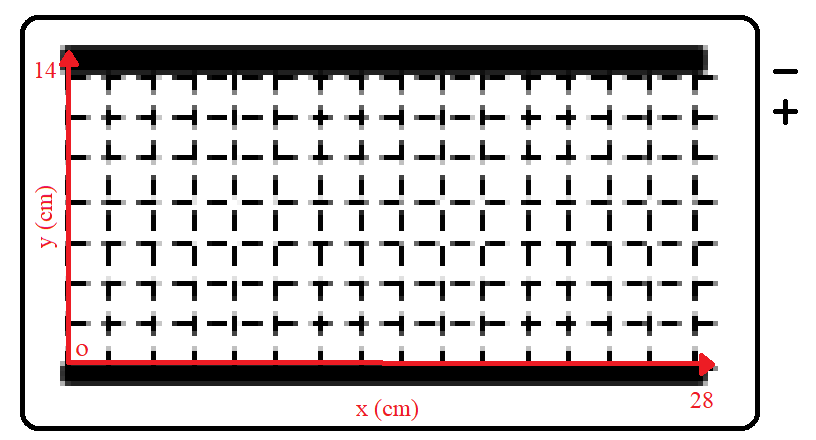
\includegraphics[width = 9 cm]{figuras/fig1.png}
\caption{\small{Posicionamento do sistema de coordenadas $(x,y)$ no esquema experimental.}}
\label{fig:1}
\end{figure*}
%------------------------------------------
%------------------------------------------


%------------------------------------------
%----------------FIGURE--------------------
\begin{figure*}[ht!]
\centering
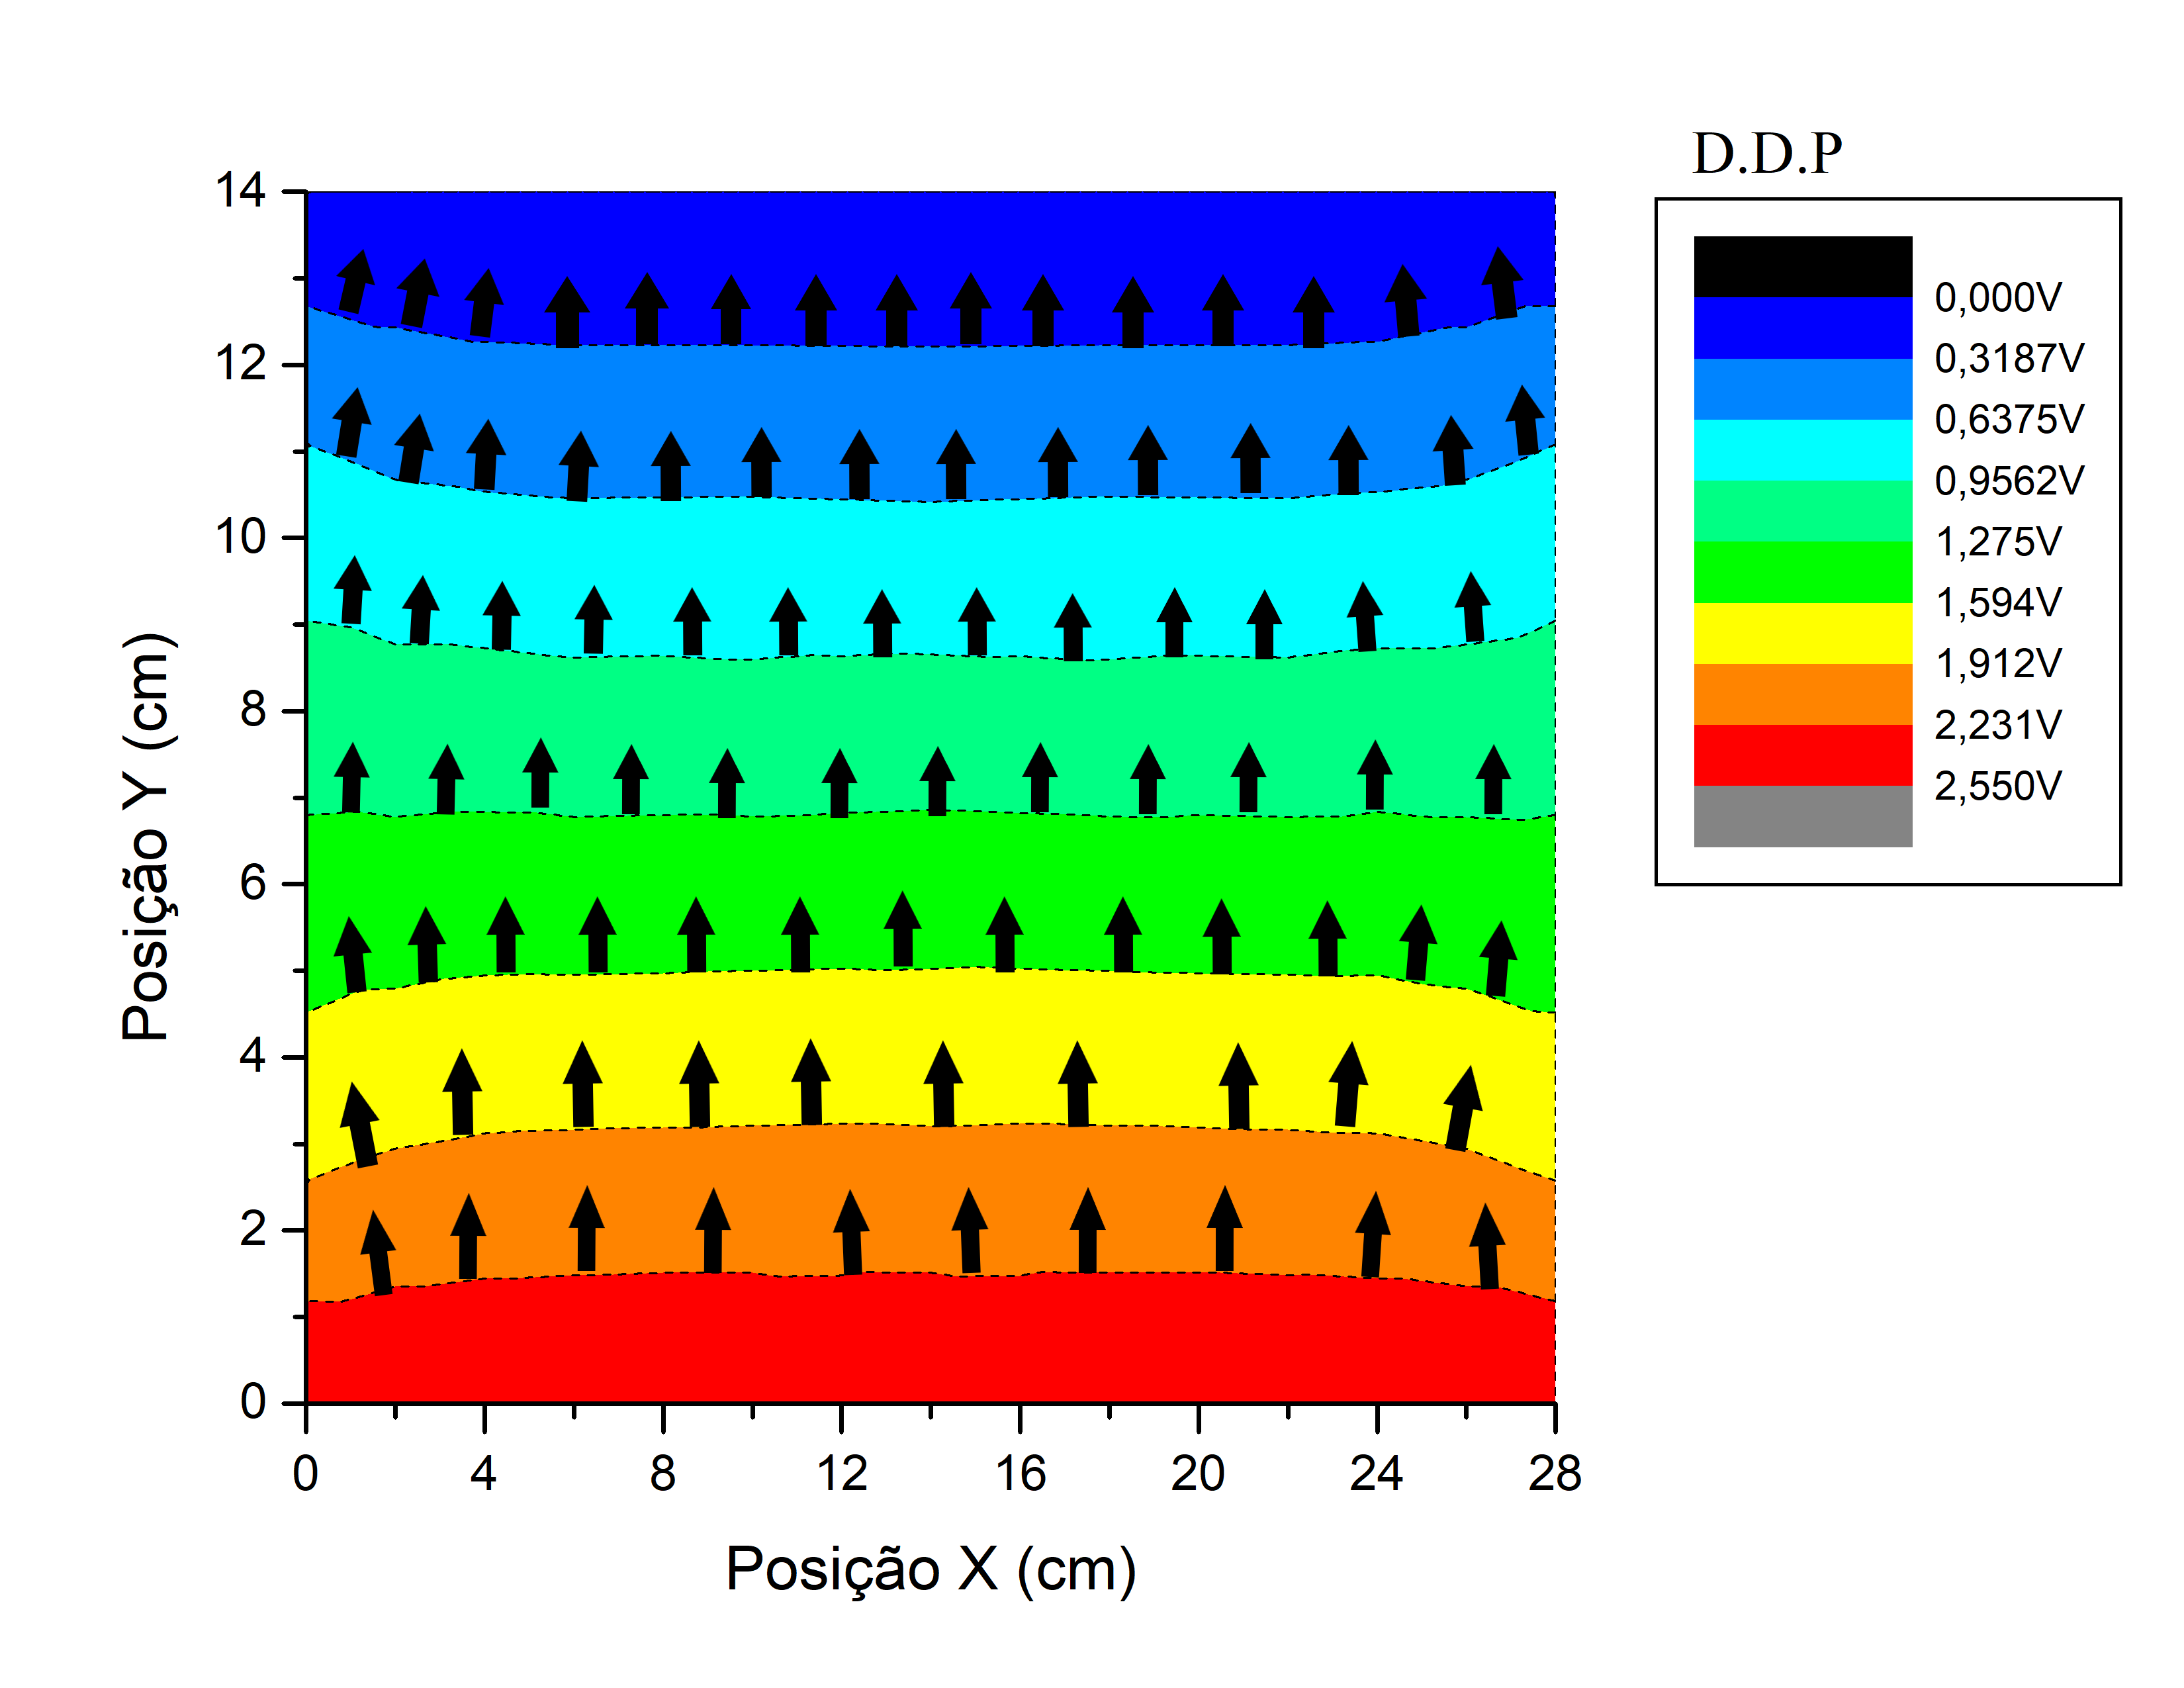
\includegraphics[width = 9 cm]{figuras/Graph5.png}
\caption{\small{Gráfico do potencial e do sentido do campo elétrico no plano com linhas equipotenciais em pontilhado do caso Figura 2(a).}}
\label{fig:2}
\end{figure*}
%------------------------------------------
%------------------------------------------

%------------------------------------------
%----------------FIGURE--------------------
\begin{figure*}[ht!]
\centering
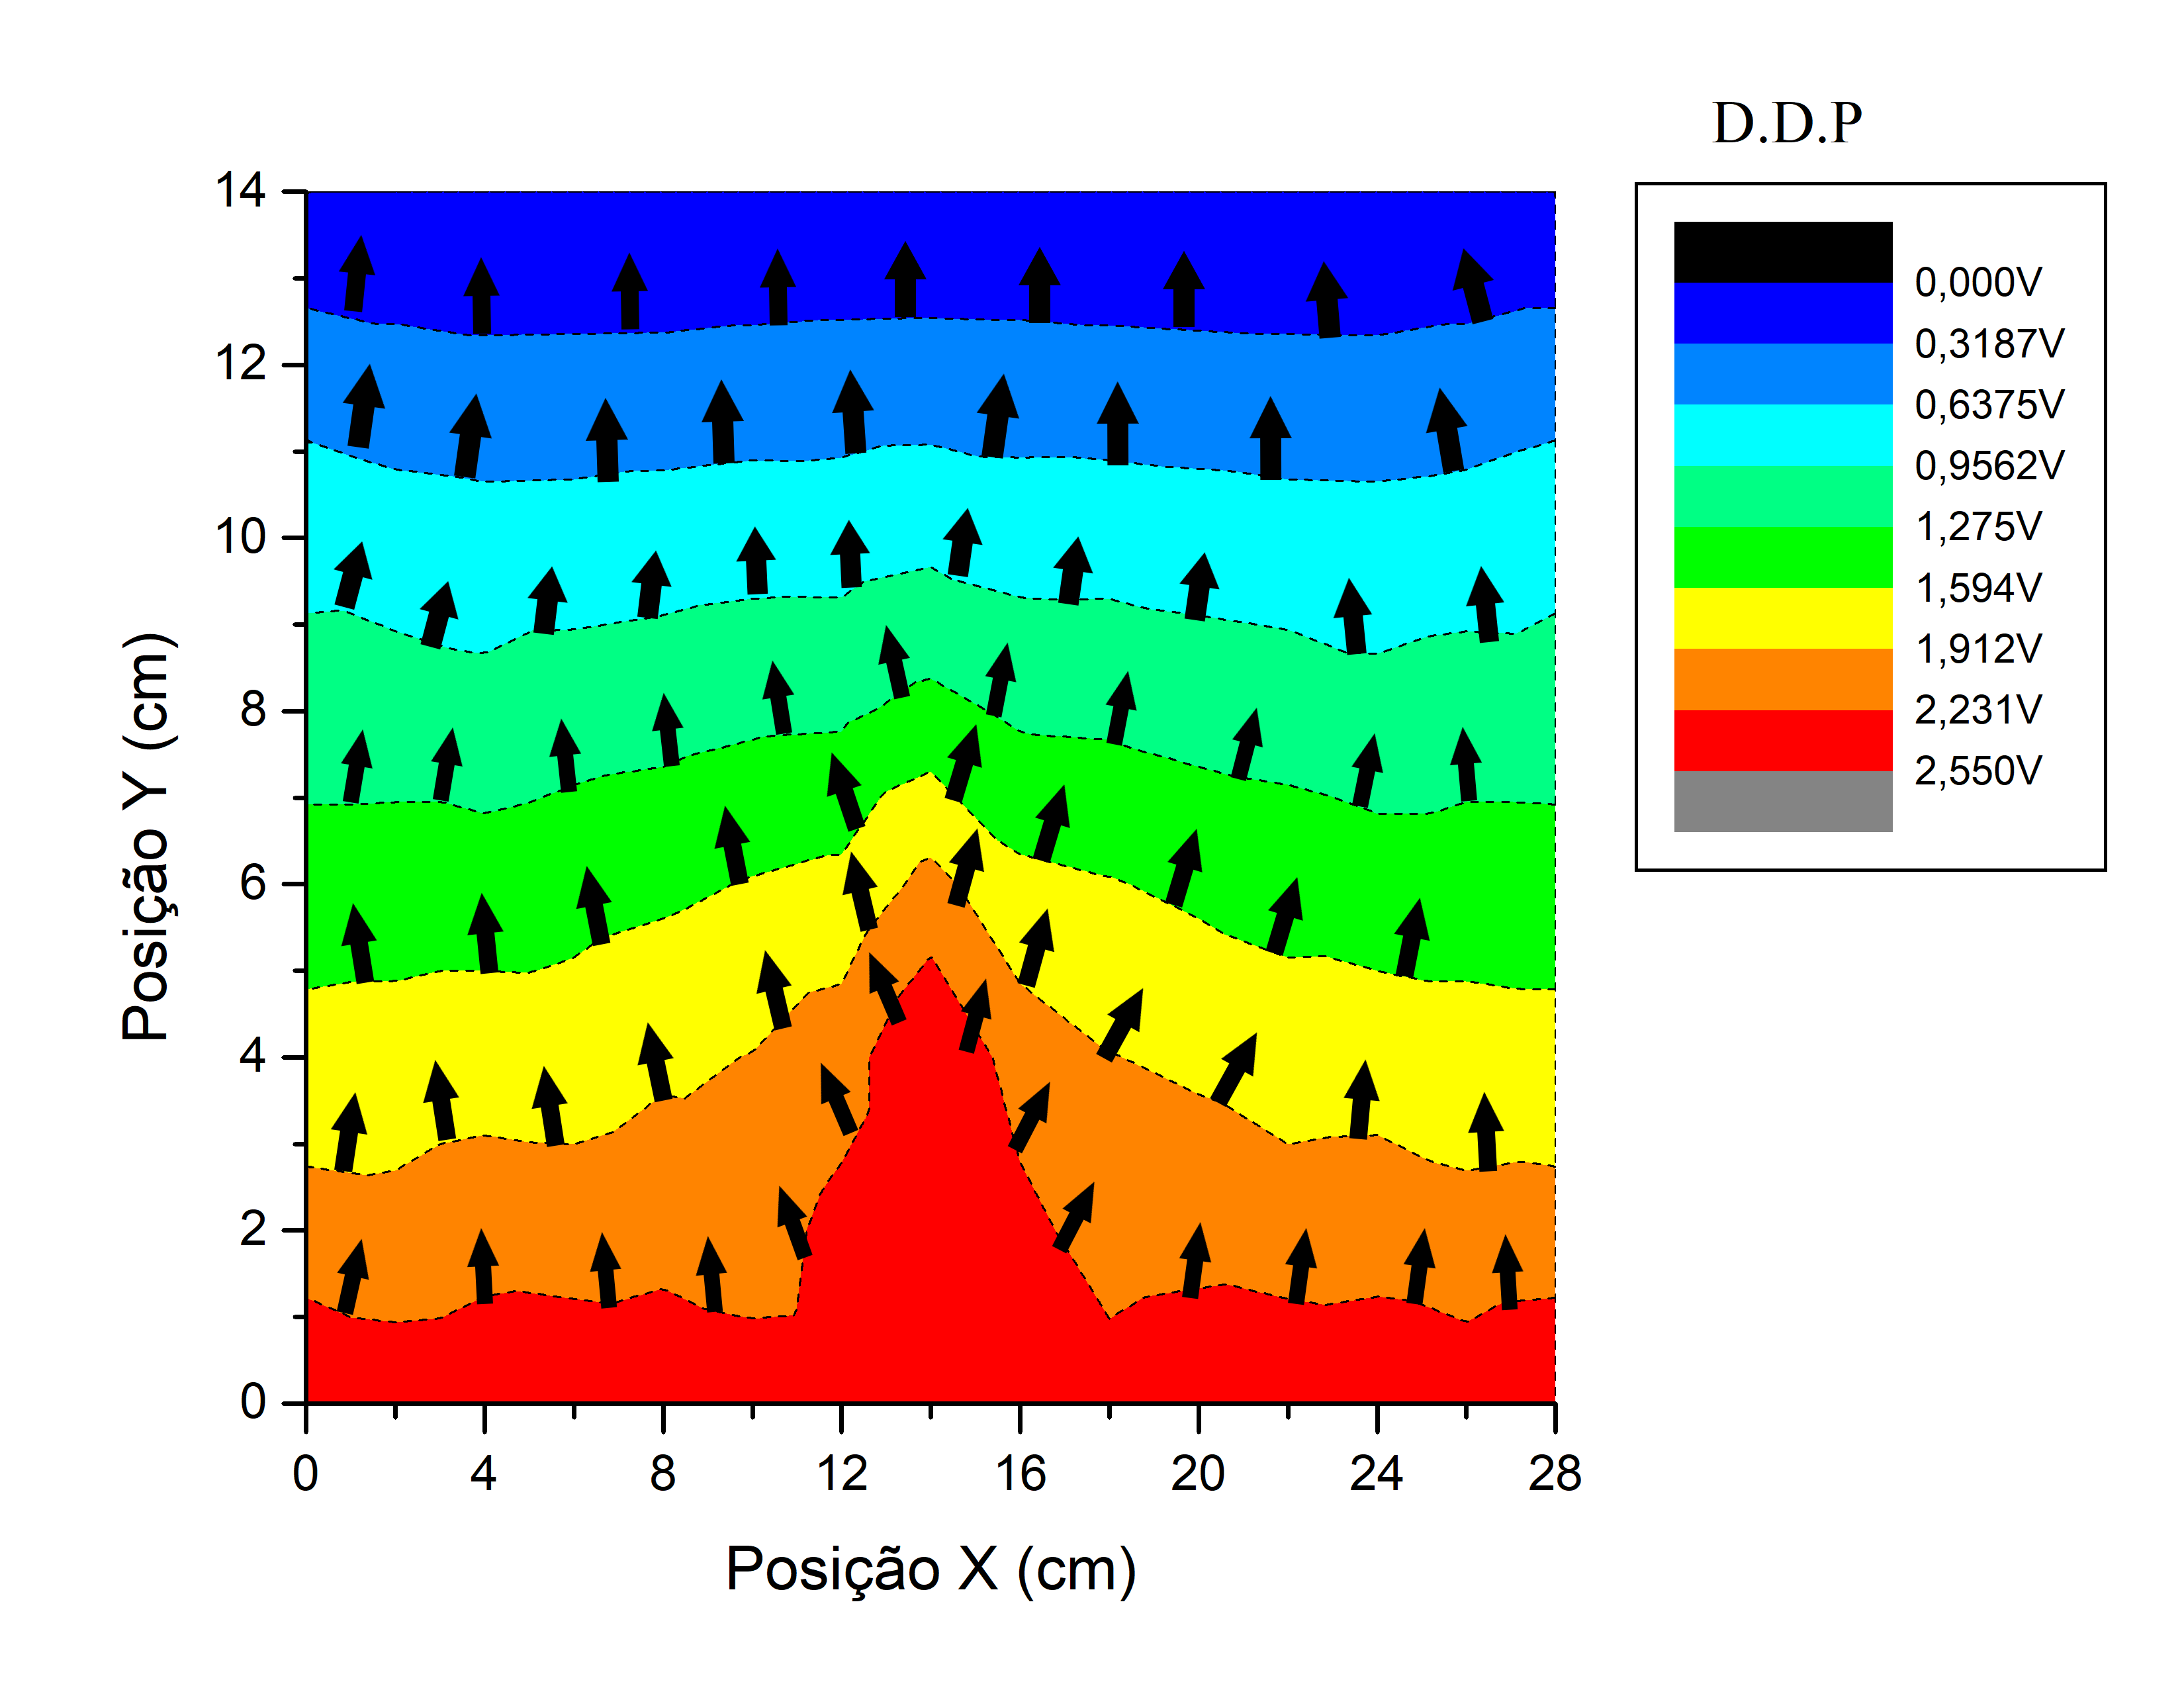
\includegraphics[width = 9 cm]{figuras/Graph4.png}
\caption{\small{Gráfico do potencial e do sentido do campo elétrico no plano com linhas equipotenciais em pontilhado do caso Figura 2(b).}}
\label{fig:3}
\end{figure*}
%------------------------------------------
%------------------------------------------

%------------------------------------------
%----------------FIGURE--------------------
\begin{figure*}[ht!]
\centering
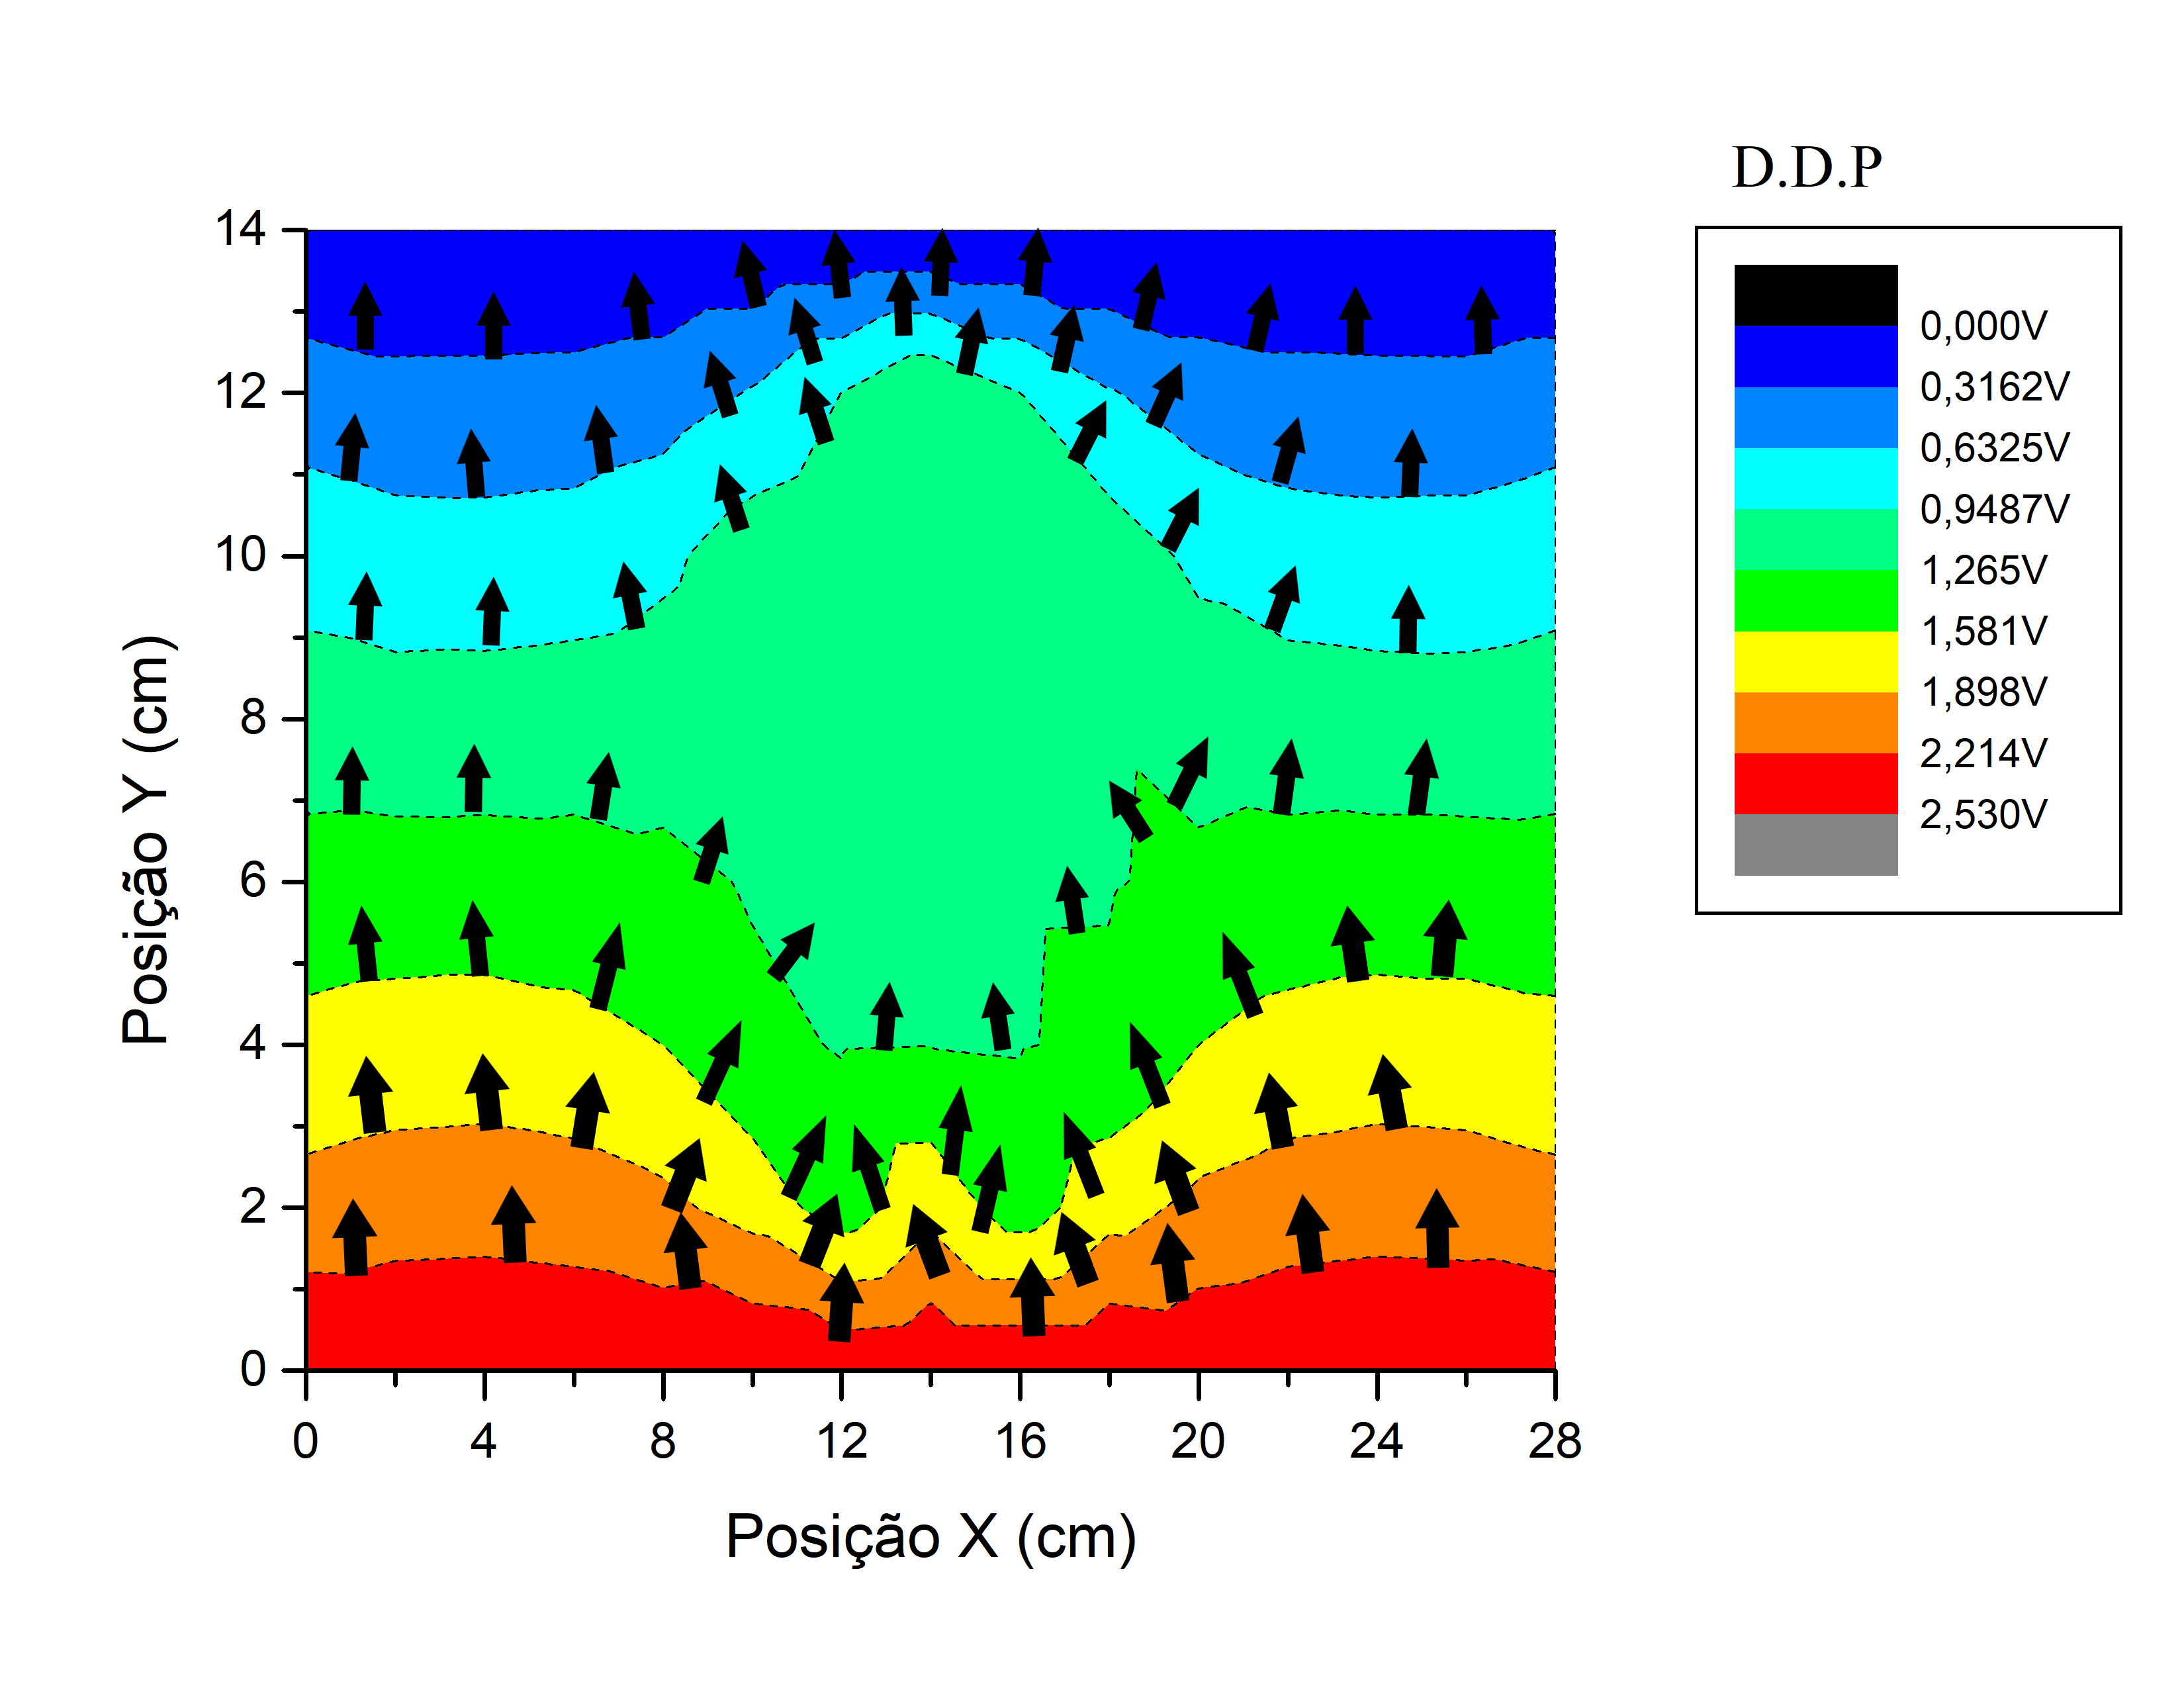
\includegraphics[width = 9 cm]{figuras/Graph1.png}
\caption{\small{Gráfico do potencial e do sentido do campo elétrico no plano com linhas equipotenciais em pontilhado do caso Figura 2(c).}}
\label{fig:4}
\end{figure*}

%------------------------------------------
%----------------FIGURE--------------------
\begin{figure*}[ht!]
\centering
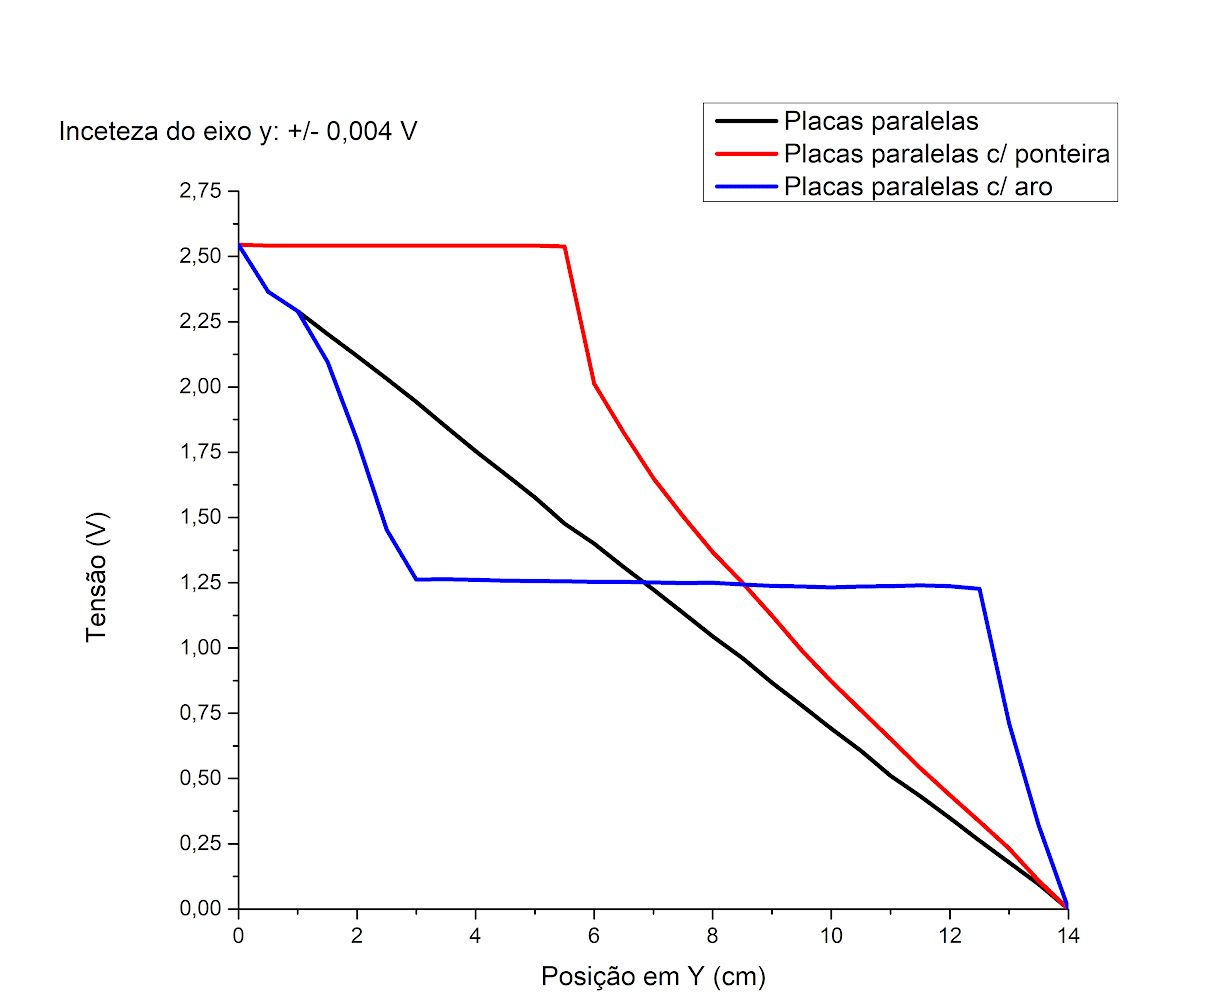
\includegraphics[width = 9 cm]{figuras/Graph6.png}
\caption{\small{Gráfico do potencial no eixo de simetria de cada uma das configurações 2(a), 2(b) e 2(c); incerteza não é visível no gráfico.}}
\label{fig:8}
\end{figure*}
%------------------------------------------
%------------------------------------------

\begin{table}[ht!]
\center
\begin{tabular}{|l|l|l|l|}
\hline
Caso & Figura 2(a) & Figura 2(b) & Figura 2(c) \\ \hline
Módulo do campo elétrico (N/C) &17.60$\pm 0.01$     & 29.20  $\pm 0.01$     & 0.40 $\pm 0.01$
\\ \hline
\end{tabular}
\caption{Módulo do campo elétrico no centro de cada caso.}
\label{tab:1}
\end{table}

Dados coletados podem ser vistos em: \url{https://docs.google.com/spreadsheets/u/1/d/1pe6sFZzzPrPHZEJ3koOhgrh1rRJFGEONfTtdWh-XQDs/edit?usp=sharing}.
%------------------------------------------
%------------------------------------------


\clearpage

%Inclui a folha de discussão de incertezas
\section{Avaliação e propagação de incertezas}

As fontes de incertezas discutidas e identificas pelo grupo foram:
\begin{enumerate}
    \item As coordenadas $(x,y)$, que dependem do posicionamento da ponteira sobre o papel milimetrado com uma f.d.p. triangular (para o papel milimetrado $a=1$ mm, incerteza padrão $u_{mili}=\frac{a}{2\sqrt{6}}=0.20$ mm). Além disso há a incerteza associada ao raio da ponteira, que foi medido como sendo $1.50\pm0.02$ mm com um paquímetro (cuja incerteza $u_{paq}$ foi calculada analogamente ao caso do papel milimetrado); essa incerteza pode ser obtida com a medida mais provável do raio ($\frac{a}{2}$) dividido por $\sqrt{6}$ por se tratar de uma f.d.p. também triangular, resultando em $u_{raio}=0.61$ mm. Combinando as incertezas obtém-se a incerteza total em cada eixo de $u_t=\sqrt{u_{mili}^2+u_{raio}^2+u_{paq}^2}=\sqrt{0.20^2+0.61^2+0.02^2}=0.64$ mm;
    \item A medida digital do voltímetro, com f.d.p. retangular e $a=0.01$ V (precisão da última casa decimal mostrada pelo voltímetro), cuja incerteza padrão é $u_V=\frac{a}{2\sqrt{3}}=0.004$ V;
    \item A influência na leitura da inclinação da ponteira em relação ao plano, que foi medida ao se inclinar a ponteira o máximo possível permitido pela distancia dos eletrodos (sem encostar nestes) ao longo da direção de maior variação do potencial, e com a ponteira fixa no centro entre os eletrodos no eixo de simetria. O valor da máxima variação foi de $0.318\pm0.006$ V (incerteza mais à frente);
    \item Foi assumido que o posicionamento dos eletrodos é ideal, isto é, um posicionado exatamente sobre o eixo $x$ e o outro paralelo a este eixo na altura $y=14$ cm, porém é observado que este não é o caso e, portanto, mais uma possível fonte de incerteza.
\end{enumerate}

A incerteza da diferença dos dois potenciais para averiguar o efeito da inclinação da ponteira é de $\sqrt{u_{V}^2+u_V^2}=0.006$, isto é, a composição da incerteza de cada medida, uma vez que a posição $(x,y)$ não foi variada.

Para o cálculo da incerteza do módulo do campo elétrico para a configuração 2(a) foi usada a seguinte fórmula:

\begin{align*}
u_{|\vec{E}|_s} &=\sqrt{\left(\frac{\partial |\vec{E}|_s}{\partial V_f} \Delta V_f\right)^{2}+\left(\frac{\partial |\vec{E}|_s}{\partial V_i} \Delta V_i\right)^{2}+\left(\frac{\partial |\vec{E}|_s}{\partial s_f} \Delta s_f\right)^{2}+\left(\frac{\partial |\vec{E}|_s}{\partial s_i} \Delta s_i\right)^{2}} \\
&=\sqrt{\splitfrac{(-(1 /(s_f-s_i)) \cdot \Delta V)^{2}+(1 /(s_f-s_i) \cdot \Delta V_i)^{2}+\left((V_f-V_i) /(s_f-s_i)^{2} \cdot \Delta s_f\right)^{2}}{+\left(-\left((V_f-V_i) /(s_f-s_i)^{2}\right) \cdot \Delta s_i\right)^{2}}} \\
&=0.0113181934 \\
&=1.13181934 \times 10^{-2} \\
&\simeq1 \times 10^{-2}
\end{align*}

Repetindo o processo para configuração 2(b), a incerteza do módulo do campo elétrico encontrada foi $1.13260493 \times 10^{-2}$, e, por último, para a configuração 2(c), o valor de incerteza do módulo do campo elétrico encontrada foi de $1.13137108\times 10^{-2}$.



\end{document}